\section{Storage \& Retreival of Dark-State Polaritons}
  \label{sec:polaritons_storage}

    We can look at the propagation of the probe pulse through the \textsc{eit}
    medium from the perspective of the atoms. Before the pulse arrives at an
    atom at a position $z$ in the medium, the atom has been optically pumped
    into the ground state $\Ket{0}$ by the coupling field. At this point the
    state is equivalent to the dark state described in equation
    \ref{eqn:lambda_eigvects}. As the leading edge of the pulse hits the atom,
    it remains in the dark state but transfers a component of its wavevector
    into a superposition between states $\Ket{0}$ and $\Ket{2}$. In this way
    energy is transferred from the probe into the medium. As the pulse reaches
    its peak and the trailing edge leaves the atom, that energy is returned to
    the pulse.

    Fleischhauer and Lukin\cite{Fleischhauer2000} introduced a useful formalism
    for describing \textsc{eit} medium with a quasiparticle known as the \textit
    {dark-state polariton}. We define a collective mixing angle $\vartheta$ via
    \begin{equation}
      \tan{\vartheta}(z, \tau) = \frac{\sqrt{Ng}}{\Omega_D(z, \tau)}
    \end{equation}
    and then the dark polariton field envelope $\Omega_D$ is given by
    \begin{equation}
      \Omega_D(z,\tau) = \cos{\vartheta}(z, \tau)~\Omega_p(z, \tau) - 
        \sin{\vartheta}(z, \tau) ~ \sqrt{Ng} \rho_{20}(z, \tau).
    \end{equation}
    The dark-state polariton quasiparticle thus describes the propagation in
    terms of a coherent mixture of the electromagnetic field with atomic spin
    wave excitation. 

    The collective mixing angle tells us how much of the polariton is stored in
    the field and how much in the spin wave. For a mixing angle $\vartheta = 0$,
    all of the energy is in the field. For $\vartheta = \pi/2$, all of polariton
    energy is in the spin wave.
    
    In the linear regime and on resonance it can be shown\cite{lambropoulos2007fundamentals} that
    $\Omega_D$ obeys 
    \begin{equation}
      \left[ \frac{\partial}{\partial t} + c \cos^2 \vartheta 
      \frac{\partial}{\partial z} \right] \Omega_D = 0,
    \end{equation}
    a wave equation describing a shape-preserving propagation with group
    velocity $v_g = c \cos^2 \vartheta$.

    % \begin{subequations}
    % \begin{align}
    %   \Omega_p &= \cos{\vartheta} \Omega_D \\
    %   \sqrt{Ng} \rho_{20} &= -\sin{\vartheta} \Omega_D
    % \end{align}
    % \end{subequations}

  \subsection{Storage \& Retrieval}

    \begin{figure}[]
      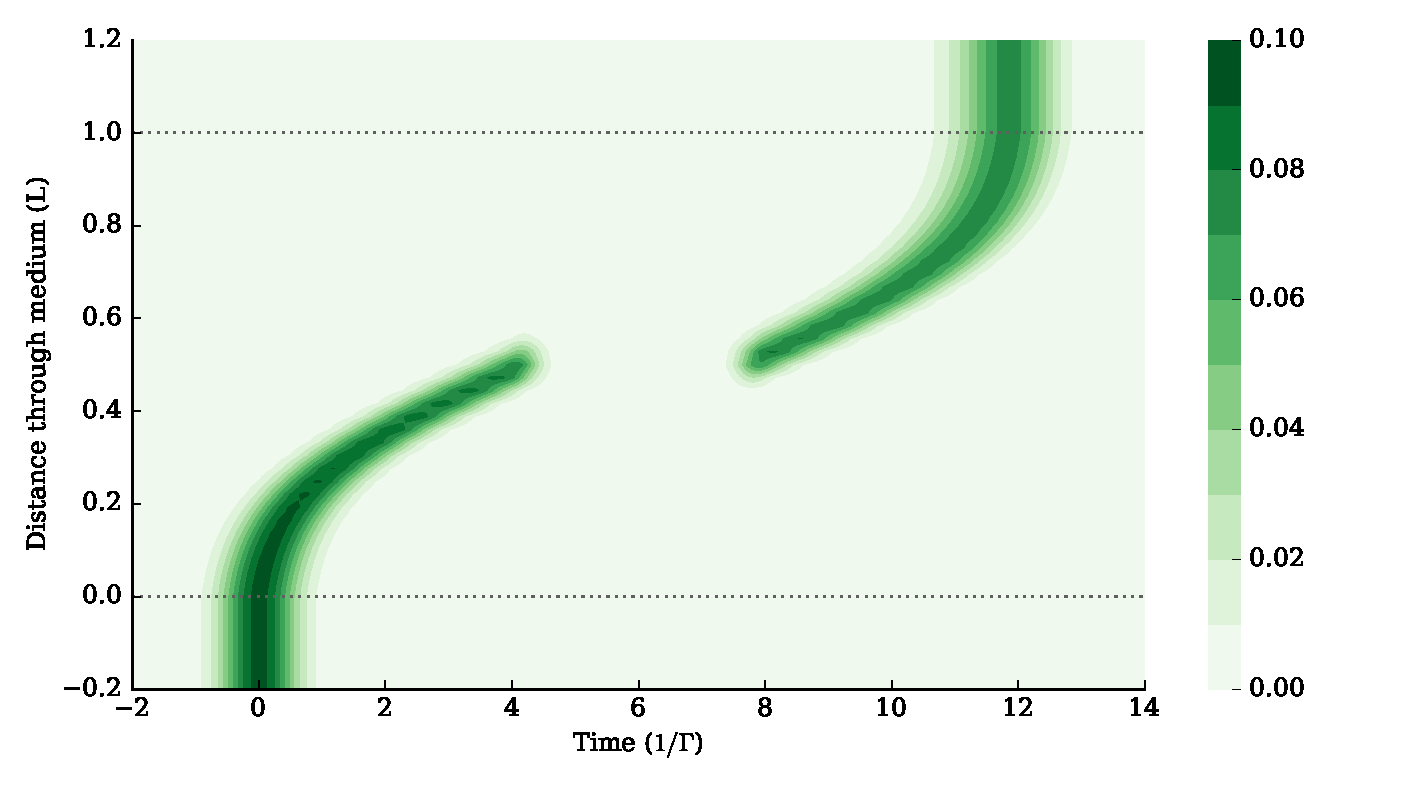
\includegraphics[width=\linewidth]
        {figs/04_polaritons/pls_p0_2pi_t1_Ng5e3_c10_gaussian_w0_5_storage_4_fig1.pdf}
      \caption{
        Simulated absolute value of $\Omega_p(z, \tau)$ for the propagation of a
        Gaussian pulse with area $\theta_p = $ \unit[0.2]{$\pi$} and
        \textsc{fwhm} $\tau_w = $ \unit[1]{$\tau_\Gamma$} through the same
        $\Lambda$-type medium as in figure \ref{fig:pulse_compression}.
        In this simulation the \textsc{cw} coupling field with $\Omega_c = $
        \unit[$2\pi~10$]{$\Gamma$} is ramped down at  \unit[4]{$\tau_\Gamma$}
        and ramped up again at \unit[8]{$\tau_\Gamma$}.
      }
      \label{fig:eit_storage}
    \end{figure}

    In figure \ref{fig:eit_storage} we show the results of the simulated
    propagation of the same probe pulse as we considered in figure
    \ref{fig:pulse_compression}, a Gaussian with area $\theta_p = $
    \unit[0.2]{$\pi$} and \textsc{fwhm} $\tau_w = $ \unit[1]{$\tau_\Gamma$}. The
    $\Lambda$-type medium also has the same non-uniform density, having a
    Gaussian profile of \textsc{fwhm} \unit[0.5]{L} and a peak density such that
    $N_{\mathrm{max}} g = \unit[2\pi~500]{\Gamma/L}$.

    The difference in this case is that the coupling field is time dependent,
    being ramped down (see equation (\ref{eqn:rampup})) over a period of
    \unit[0.5]{$\tau_\Gamma$} at $t' = $\unit[4]{$\tau_\Gamma$} and ramped up
    again at $t' = $\unit[8]{$\tau_\Gamma$}.

    We see that the effect is that the pulse envelope vanishes as the coupling
    field is ramped down, but returns dramatically, with the same profile, as
    the coupling field is ramped back up. It appears as though the light has
    been `stopped' by the medium before being allowed to continue on its way. 

    We can understand this behaviour by considering the propagation of the dark
    state polariton in this system. Ramping down the driving field envelope
    $\Omega_c$ once the pulse is in the medium equates to rotating the mixing
    angle $\vartheta \rightarrow \pi/2$ such that it is coherently mapped on to
    the spin wave. At a time later, in this case $t' = $\unit[8]{$\tau_\Gamma$},
    we ramp up the driving field, rotating the mixing angle back to its previous
    position, and the field continues on its way. This excitation transfer can
    be seen in figure \ref{fig:dark_state_components} which shows the separate
    components of the dark state field.

    Although the storage and retrieval of dark-state polaritons is often
    described as `stopping light', we must be careful to note that it is really
    a coherent transfer of energy to the medium. No elecromagnetic field
    envelope remains at the limit $\vartheta = \pi/2$, so the light itself is
    not `stopped', it has been transferred into a spin excitation.\cite{Fleischhauer2000}

    \begin{figure}[]
      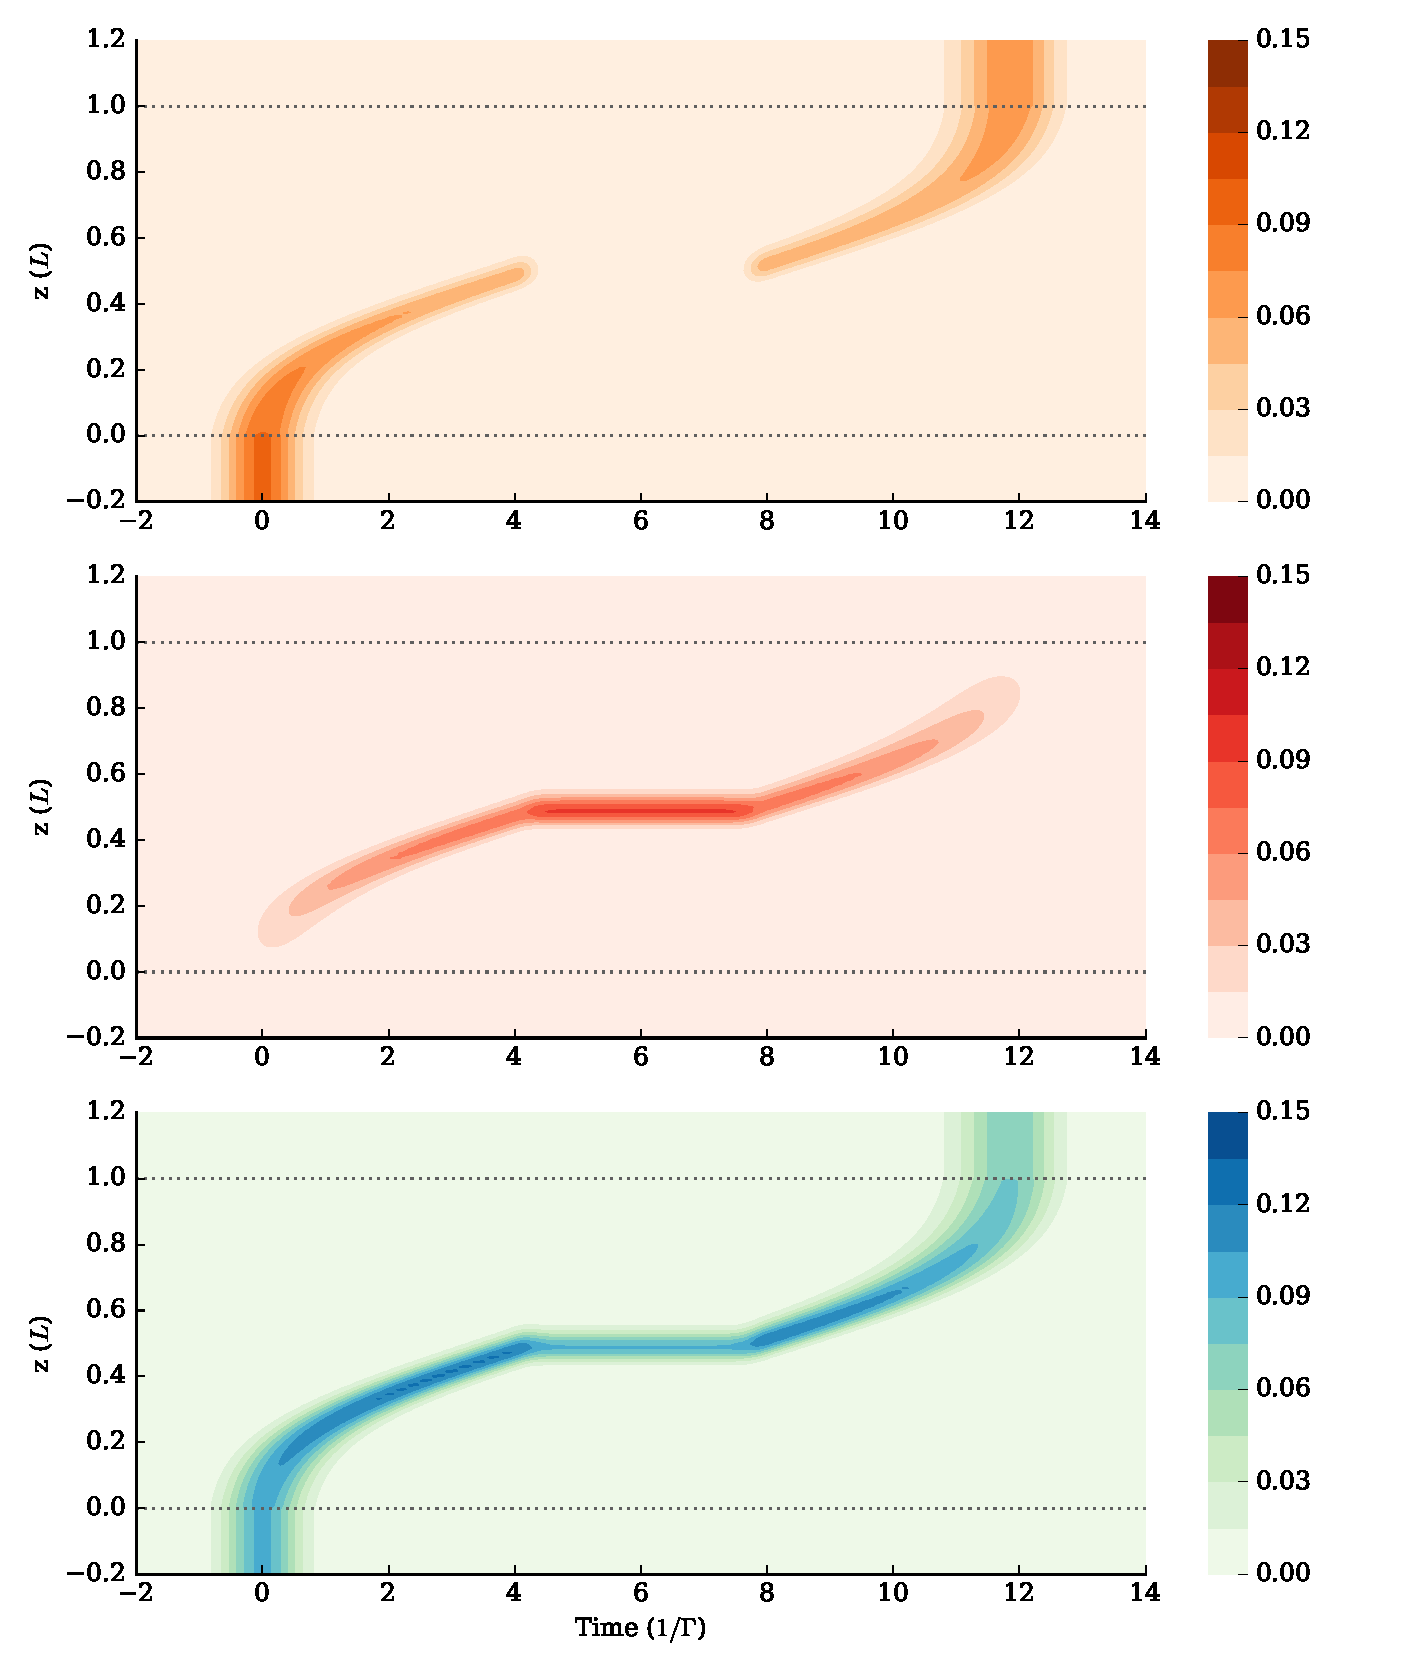
\includegraphics[width=\linewidth]
        {figs/04_polaritons/pls_p0_2pi_t1_Ng5e3_c10_gaussian_w0_5_storage_5_fig4.pdf}
      \caption{
      Dark state polariton components for the storage and retrieval simulation
      in figure \ref{fig:eit_storage}. (Top) The field component
      $\cos{\vartheta}(z, \tau)~\Omega_p(z, \tau)$. (Middle) The spin wave
      component $-\sin{\vartheta}(z, \tau) ~ \sqrt{Ng} \rho_{20}(z, \tau)$.
      (Bottom) The total dark state field $\Omega_D(z,\tau)$.
      }
      \label{fig:dark_state_components}
    \end{figure}

  % \subsection{Inhomogeneous Broadening}

  % - (possibly Doppler broadening)

    It is important to consider the limitations of these techniques. First, for
    \textsc{eit} and associated slow light effect, the duration of the pulse
    $\tau_w$ must be greater than the reciprocal of the \textsc{eit} bandwidth,
    so that spectrally it propagates in the transparency   window. Second, for
    storage of the entire pulse to be possible, the spatial extent of the pulse
    must be compressed below the length $L$ of the medium, which is possible
    only if the medium has a sufficiently large optical depth such that $Ng L
    \gg 1$.\cite{Fleischhauer2005}

  The first demonstrations of this storage and retrieval technique were made by
  Liu \etal \cite{Liu2001} and Phillips \etal\cite{Phillips2001}, in which
  pulses were stored for much longer than the pulse duration. Recent
  developments in ultracold atomic systems have pushed storage records up to the
  order of a minute.\cite{Dudin2013}


  % - applications (see qu memory review)